\Chapter{Optimalizálás}

\section{Probléma kifejtése}
Mikor az alkalmazás hozzávetőlegesen elérte végső fázisát, és a funkciók nagy része működött, akkor derült fény arra a problémára, amit már előre lehetett sejteni, ez pedig a futási idő.
Mivel nagyon sok számítást kell elvégeznie a programnak, így elkerülhetetlen, hogy lassabban működjön az alkalmazás. Ebben a fejezetben ezt a problémakört fejtem ki.

A lassúság funkcionális problémát nem okoz, mivel a célként kitűzött feladatokat a program elvégzi. Ez inkább a felhasználási mód rovására megy. Az alap elképzelés ugyanis úgy szólt, hogy egy olyan végeredményt kapok, amit egy asztalnál, élő pókerezés közben úgynevezett csaló szoftverként tudok használni, ami elvégzi a gondolkodást helyettem. Hogyha 30 percet kell várni arra, hogy a flop-on kiszámolja a program, milyen esélyeim vannak, akkor azt a gyakorlatban nem lehet effektíven felhasználni.

\section{Lehetőségek vizsgálata}
Ahhoz, hogy optimalizálni tudjam az alkalmazást, először meg kell vizsgálni, mi okozhatja a lassulást, vagy hol lehet változtatni a kódon. A leginkább akkor szembetűnően lassú a program, mikor az ellenfél esélyeit vizsgálom. Ezért optimalizálási szempontból kizárólag a back end-re, azon belül is leginkább a findEnemyStrongest.js forráskódjára fókuszáltam.

Az alábbiakban felsorolom azokat a tényezőket, amiket változtatni terveztem a program gyorsítása érdekében. Ezeket később pontról pontra kifejtem, bemutatva az eredeti és a módosított megoldásokat, valamint megpróbálom szemléltetni az elért gyorsulást, amennyiben tapasztalható egyáltalán.
\begin{itemize}
    \item Adathalmaz átszervezése: Mivel az adathalmazban az elemek kártya értékek szerint voltak sorba rendezve, így eszerint kellett rendeznem az asztalon lévő lapokat is. Ehelyett ABC sorrendbe rendezem a gyorsabb keresés érdekében.
    \item Tömbök előre allokálása és indexelése: Mivel az, hogy adott esetben hány értéket kapunk az ellenfél lehetséges lapjaira, ismert, ezért ahelyett, hogy minden esetben push-olok egy értéket a tömbbe, inkább előre definiálom és az aktuális elemet mindig hozzáadom.
    \item Függvények kiszervezése: Alap esetben nem túl esztétikus, ha a default függvényben több soros programkódok vannak. Ezen kívül úgy gondoltam, gyorsulni fog a program, ha amit csak lehetséges külön függvénybe szervezek, amit utána csak meg kell hívnom.
\end{itemize}

\section{Optimalizálás megvalósítása}

\subsection{Adathalmaz átszervezése}
Az adathalmazom alapvetően kártyaértékek szerint volt rendezve. Egyrészt azért, mert a forrásban is így volt tárolva, másrészt az emberi szem számára is könnyebben értelmezhető így. Tehát a royal flush megfelelője a "AKQJTF" volt, az F azt jelöli, hogy figyelembe kell venni, hogy egyező színűek a lapok. Mivel az adathalmazban így voltak rendezve az elemek, az aktuálisan kiválasztott lapokat is ilyen módon kellett sorba állítanom. Első körben logikusnak tűnt ez a megoldás, viszont a megvalósítása kicsit hosszú programkódot eredményezett. 

\begin{lstlisting}[style=htmlcssjs]
function sortCardOrder(string, colors) {
  let ordered = "";
  let timesArray = [
    (string.match(/A/g) || []).length,
    (string.match(/K/g) || []).length,
    .
    .
  for (let i = 0; i < timesArray[0]; i++) {
    ordered += "A";
  }
  for (let i = 0; i < timesArray[1]; i++) {
    ordered += "K";
  }
  .
  .
  if (colors["C"] == 5) {
    ordered += "F";
  } else if (colors["H"] == 5) {
    ordered += "F";
  } else if (colors["S"] == 5) {
    ordered += "F";
  } else if (colors["D"] == 5) {
    ordered += "F";
  }

  return ordered;
}
\end{lstlisting}

Látható, hogy mind a 13 lapot külön kellett vizsgálnom, és úgy összefűzni egy string-é. A függvény végén az egyező színeket számolom össze, amennyiben létezik olyan lehetőség, hogy 5 egyforma színű kártya van, akkor hozzáfűzök a string végére egy "F"-et.

Először az adathalmazt kellett módosítanom. Mindössze annyi történt, hogy az elemek nem értékek szerint lettek sorba rendezve, hanem ABC sorrend szerint. A fenti példánál maradva, így a "AKQJTF"-ből "AFJKQT" lett. Ennek köszönhetően nem volt szükség az összes kártyát külön vizsgálnom.

A módosított függvény elején szintén vizsgálom a színeket, viszont utána már csak beépített függvényeket használok. A sorba rendezésre a sort() függvény használható, viszont az csak egy tömb elemeit rendezi sorba, nekem viszont az elemek betűit kell sorba rendeznem. Éppen ezért használom még a split(), illetve a join() függvényeket. Az előbbi feldarabolja az elemeket jelen esetben karakterekre, hogy azokat tudjam rendezni. Az utóbbira azért van szükség, hogy a feldarabolt, sorba rendezett értékeket újra összefűzze string-ekké, így ugyanannyi elemű tömböt kapunk vissza, mint ahány elemű a függvények hívása előtt volt. 

\begin{lstlisting}[style=htmlcssjs]
function sortCardOrder(string, colors){
    let ordered = string;
    if(colors['C'] == 5){
      ordered+='F'
    } else if(colors['H'] == 5){
      ordered+='F'
    } else if(colors['S'] == 5){
      ordered+='F'
    } else if(colors['D'] == 5){
      ordered+='F'
    }
  
    return ordered.split('').sort().join('');
}
\end{lstlisting}

\subsection{Tömbök előre allokálása és indexelése}
A tömbök létrehozására a push függvényt használom. Minden lehetséges lapkombináció kiszámításánál ezzel a függvénnyel töltöm fel a tömböket, amikkel majd visszatérek és átadom a front end-nek. Ezt a függvényt, például flop-on az ellenfél esélyeinek számításánál 1.070.190-szer hívom meg. Az volt a feltevésem, hogy ez a módszer lényegesen lassítja a szoftver működését.

Mivel minden vizsgálatnál adott, hogy hány elemű lesz a tömb, így meg lehet oldani, hogy a tömböket előre allokálom. Az elágazások elején definiálom a tömböket, hogy hány eleműek legyenek, majd a feltöltéskor mindig az éppen aktuális elemet hozzá fűzöm ehhez a tömbhöz. A vizsgálatoknál több helyen foreach ciklust használok, ennek a hátránya, hogy nem tudom a tömböket indexelni. Hogyha előre allokálom a tömböket, akkor szükségem van az indexelésre. Ennek érdekében azokon a helyeken, ahol meg szeretném ezt valósítani át kell alakítanom a foreach ciklusokat egyszerű for ciklusokká.

Hogy minél kevesebb programkódot kelljen bemutatnom, kizárólag azokat a részleteket szemléltetem, amikor mindegyik kártya ki van osztva, ugyanis ilyenkor a legrövidebb a kód. Alább látható ennek az optimalizálás előtti változata.

\begin{lstlisting}[style=htmlcssjs]
  let result = [];
  if (sevenCards.length == 7) {
    let eCombination = createEnemysPossibleHands(everyCards, sevenCardsName);
    for (const comb of eCombination) {
      result.push(findStrongestOfEnemysCards(comb));
    }
    return result;
  }
\end{lstlisting}

Ezek alapján az elágazás előtt nem csak definiáltam a result tömböt, hanem meg is határoztam a méretét. Mikor ez megvolt, át kellett alakítanom a belső foreach ciklust, hogy az indexelést el tudjam végezni. Ennek a két feltételnek kellett teljesülnie, hogy megvalósítsam az optimalizálásnak ezt a tényezőjét.

\begin{lstlisting}[style=htmlcssjs]
  let result = new Array(990);
  if (sevenCards.length == 7) {
    let eCombination = createEnemysPossibleHands(everyCards, sevenCardsName);
    for (let i=0; i<eCombination.length; i++) {
      result[i] = findStrongestOfEnemysCards(eCombination[i])
    }
    return result;
  }
\end{lstlisting}

\subsection{Függvények kiszervezése}
A default függvényemben és azon kívül is sok helyen nagyon hosszú programkódok szerepeltek. A terv az volt, hogy ezeket külön függvényekbe szervezem ki. Egyrészt gyorsulást reméltem ettől, másrészt esztétikai és átláthatósági problémákat okoz, ha egy nagy, ömlesztett kódból áll az egész program.

Próbáltam minél rövidebb kódot kapni, ennek érdekében az első lépésem az volt, hogy megvizsgáltam melyek azok a programrészletek, amelyeket a findStrongest.js és a findEnemyStrongest.js file-ban is felhasználok. Létrehoztam a helperFuncitons.js-t, amibe kiszerveztem ezeket a részleteket külön függvénybe, majd a többi file-ba már csak importálnom kellett és fel is tudtam használni. Az alábbi kódokat szerveztem ki külön függvénybe és helyeztem a helperFuncitons-js-be:
\begin{itemize}
    \item removeItemOnce(): Ez a függvény megkap egy tömböt és egy értéket, majd kitörli a kapott tömbből a kapott értéket, ezután visszatér a szűkített tömbbel.
    \item sortCardOrder(): Ez az adathalmaz átszervezésénél tárgyalt függvény. Eleinte ez is ömlesztve, ismétlődve szerepelt mind a két file-omban. Az optimalizált változatot is kiszerveztem.
    \item getOnlyName(): Front end-en egy objektumban tárolom azokat a kártyákat, melyeket kiválasztott a felhasználó. Back end-en az objektumból csak egy értékre van szükségem, a kártyák neveire, azt viszont egy tömbben is el tudom tárolni. Ez a függvény pont ezt hivatott megvalósítani. Szintén a helperFuncitons.js-be került.
    \item getJustDeck(): Ez egy gyakran használt részlet. Megkapja az összes kártyát, valamint a kiválasztott lapokat. Visszatér ennek a különbségével, tehát a pakliban maradt kártyákkal.
\end{itemize}

A közös részek kiszervezésével lényegesen rövidebb lett a programkód. Ezután az összes file-ban igyekeztem a default függvény hosszát a minimumra csökkenteni. A leginkább szembetűnő változás a findStrongest.js default függvényében történt. Az optimalizálás előtt 80 soros volt ez a függvény, a végére pedig sikerült lecsökkenteni 30 sorosra. Ezt az összesen 110 sor programkódot nem szemléltetném, inkább csak a leglényegesebb részt. Az eddigi 2 külön függvényből lett 5, amiből a legtöbb változást a createStrongest függvény hozta.

\begin{lstlisting}[style=htmlcssjs]
function createStrongest(combinations){
  let rawdata = fs.readFileSync("data.json");
  let strenghtOrder = JSON.parse(rawdata);
  let result =  [];
  for (let combination of combinations) {
    let nameString = "";
    let colors = { C: 0, S: 0, H: 0, D: 0 };
    for (let card of combination) {
      nameString += card[0];
      colors[card[1]] += 1;
    }
    let ordered = sortCardOrder(nameString, colors);
    result.push(strenghtOrder.cardStrenght[ordered]);
  }
  return Math.min(...result);
}
\end{lstlisting}

Ez a részlet valósítja meg azt, amit a felhasználó magától is el tud dönteni. Megkap 25, 5 elemű tömböt, ezek a 7 lerakott lapból kiválasztható 5 lap. Ezeket mind megkeresi az adathalmazban, majd a legkisebb értékűvel tér vissza. Tehát megadja, hogy a választható 7 lap közül melyik 5 lap az, amelyik a legerősebb, ez lesz a játékosé. Ezt a keresést akkor is el kell végezni, amikor ismerjük az összes lapot, valamint akkor is, mikor csak 5-öt vagy 6-ot. Ezek alapján a default függvényben ez a részlet háromszor szerepelt. Éppen ezért sikerült ezzel elérni szembetűnően rövidebb kódot.

\section{Eredmények kiértékelése}
Annak érdekében, hogy a futási időről készült méréseim hitelesek legyenek, kitűztem néhány előfeltételt. Mivel nem ugyanannyi időbe telik a programnak elvégezni a számításokat különféle lapok esetében, így minden mérésnél azonos lapokat választottam ki, hogy a mérést pontosnak tekinthessem. Ezek a következőek voltak. Saját lapjaimnak a pikk ászt, és pikk királyt választottam. A flop a pikk ász, pikk 10-es, és pikk 2-es volt. Turn-ön a treff 10-es, majd végül river-nél a treff 7-es. Minden mérésnél ezeket a lapokat választottam ki, illetve mindig az éppen aktuálisakat. Természetesen a flop vizsgálatánál a saját lapjaimon kívül csak három lapot raktam le az asztalra.

Másik tényező, amit fontosnak tartottam egységesíteni az a hardver, amin futtatom az alkalmazást. A méréseket ugyan azon a számítógépen végeztem. Csak a kliens, a szerver, és a böngésző futott a gépen, ezzel is elősegítve azt, hogy más, háttérben futó alkalmazás nem befolyásolja a mérést. 

\begin{figure}[ht]
\centering
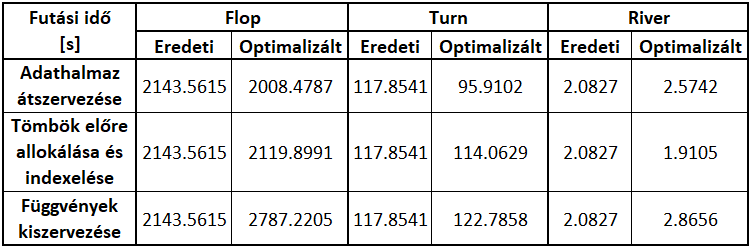
\includegraphics[scale=0.85]{images/running-time.png}
\caption{Futási idők módosításonként}
\label{fig:running-time}
\end{figure}

A 4.1-es ábrán láthatóak a futási idők mind a három módosításra levetítve, valamint a preflop utáni licitkörökre. Mint azt az ábra is jól mutatja, sajnos nem sikerült a várt gyorsulást elérni, viszont érdekesek az eredmények, amiket kaptam.

A legnagyobb javulást az adathalmaz átszervezésével értem el. A river-nél egy fél másodperces lassulás tapasztalható, viszont a turn esetében már 22 másodperces javulást látunk. Futási idő szempontjából a flop a legkritikusabb, itt pedig több, mint két perces javulást eredményezett a módosítás. Ebből a szempontból elhanyagolható, a fél másodperces lassulást river-nél, hiszen az kevésbé feltűnő a felhasználónak, mint a flop számításának lassúsága.

A tömbök előre allokálása és indexelése minimális javulást hozott. River esetében megközelítőleg egy tizedmásodperces, turn-nél 3 másodperces, flop-nál pedig 24 másodperces gyorsulást tapasztaltam. Ezek alapján elmondható, hogy a push függvény nem lassítja lényegesen a futási időt.

Nagyon érdekes, hogy a függvények kiszervezése nemhogy gyorsulást nem eredményezett, de kifejezetten lassította a programot. A lehetőségek vizsgálata alszakaszban is látható, hogy két fő célom volt ennek a megvalósításával, a futási idő javítása jól láthatóan nem volt sikeres. A másik célom viszont a programkód jobban olvashatóvá és esztétikusabbá tétele volt. Flop esetében több, mint 10 perces lassulást hozott a függvények kiszervezése. Alap esetben nem kellene érezhetőnek lennie, hogy egy programrészletet közvetlen futtatunk, vagy egy külön függvénybe írjuk és úgy hívjuk meg. Az én esetemben viszont, a flop-nál maradva, ezt a függvényt 1.070.190-szer kell meghívnom. Valószínűleg ha ennyiszer hívunk meg egy függvényt, akkor ott már szembetűnő lesz ez az időtartam, ez okozhatja jelen esetben is a lassulást. Ezeket figyelembevéve két lehetőségem volt, az egyik, hogy elvetem ezt a megoldást és a default függvényben marad ugyan az a programkód többször is. A másik, hogy elfogadom az ezzel járó lassulást, cserébe esztétikusabb lesz a kódsor. Mivel nem tervezem az alkalmazást publikálni, így inkább amellett döntöttem, hogy a szakdolgozatom szempontjából hasznosabb, ha inkább az átlátható programkód mellett döntök.

\section{Működés ellenőrzése}
Az alkalmazás véleményem szerint elérte végső formáját. Nem maradt más hátra, mint a tesztelés, hogy megbizonyosodjak, az alkalmazás rendben működik. Ehhez, a szakdolgozat elején említett hasonló szoftverek egyikét hívtam segítségül. Azt választottam, amelyikben ki lehet választani azt, hogy hány játékossal játszunk. A szoftver alap működését meglehetősen egyszerűen lehet tesztelni ennek a segítségével. Mindössze annyit kell megvizsgálnom, hogy az általam készített program ugyanazt a százalékos végeredményt adja-e, mint az interneten találté.

Többféle leosztást is összehasonlítottam, mindenhol ugyanazt az eredményt kaptam, viszont jelen esetben csak egyet szemléltetnék. Próbáltam a lapokat véletlenszerűen kiválasztani. Jelen esetben a felhasználó lapjai, a káró 7-es, és 2-es. A flop a treff 7-es, kör 2-es, és a treff ász. Így tehát két párunk alakult ki, ami kifejezetten jó eset, azaz magas nyerési esélyre számíthatunk. A Pokerstars által szponzorált alkalmazás azt a végeredményt adta, hogy 84,87\% esélyünk van nyerni, az ellenfélnek pedig 13,86\%. A saját szoftveremnél ugyanezeket a lapokat választottam ki. Eredménynek ugyancsak 84,87\%-ot kaptam a saját nyerési esélyeimre, így az ellenfelé 100\%-84,87\%=13,86\%. Így tehát kijelenthetjük, hogy a százalékos esélyek számítása jól működik az alkalmazásomban, legalábbis flop-on.

Továbbmenve, a következő helyzet, ahol vizsgálni kell a helyes működést, az a turn. Negyedik lapnak a pikk ászt választottam. Ebben az esetben a board-on kialakult egy pár, ami a felhasználó egyik párját értéktelenné teszi, mivel az ász pár és 7-es pár sokkal erősebb, mint a 7-es és 2-es párok. Ebben az esetben az várjuk, hogy jóval kevesebb lesz a felhasználónak a nyerési esélye, mint a flop-nál volt. Az internetes szoftver most 72.62\%-ot mutat. Kiválasztottam a saját alkalmazásomban is a pikk ászt, ami így 72,6\%-ot írt ki. Látható, hogy a két program számítása között két százados különbség van. Egyrészről ez a felhasználó szemszögéből elhanyagolható, másrészt ezt a különbséget a feltételezett számítási módszereknek, valamint a lehetséges kerekítési különbségeknek tudom be. A többi esetben ilyen eltérést nem tapasztaltam.

Eddig az alkalmazás az elvártaknak megfelelően működik. A flop-nál és a turn-nél is megbizonyosodtam arról, hogy a kapott esélyek helyesek. Már csak az utolsó lap van hátra, a river, ahol a treff királyt választottam. Így három egyforma színű lap van az asztalon, ami esélyt ad arra, hogy valakinek flush-e alakuljon ki. Ezért várhatóan a játék utolsó százalékos esélye még kevesebb lesz a korábbiaknál. Az interneten futtatva 63,33\% nyerési esélyt kaptam, ami az általam elkészített verziónál is megegyezett. A fentieket figyelembe véve kijelenthető, hogy a szakdolgozatom webalkalmazása jól működik, tehát helyes értékeket számol. A 4.2 és 4.3 ábrán szemléltetem a két alkalmazás számolt értékeit river esetén.

\begin{figure}[ht]
\centering
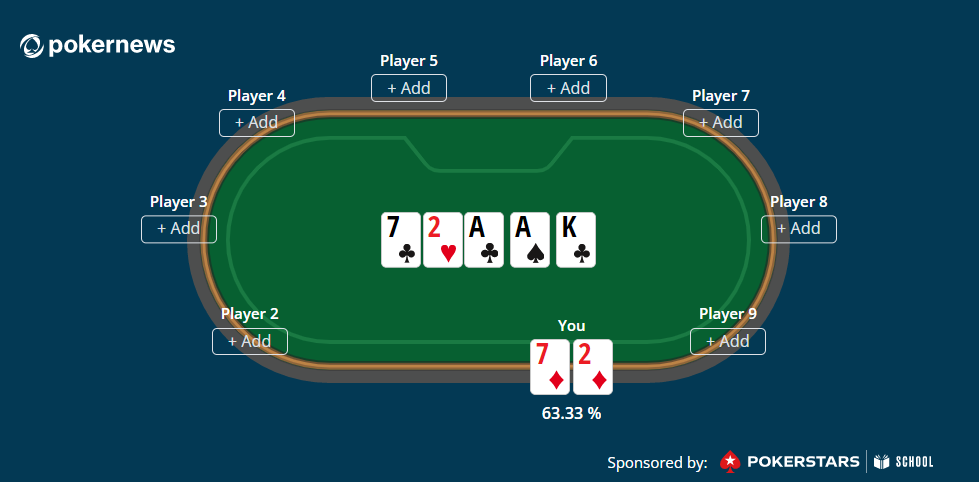
\includegraphics[scale=0.7]{images/test-ps.png}
\caption{A Pokerstars alkalmazásának számítási eredménye river-nél \cite{pokerstars}}
\label{fig:test-ps}
\end{figure}

\begin{figure}[ht]
\centering
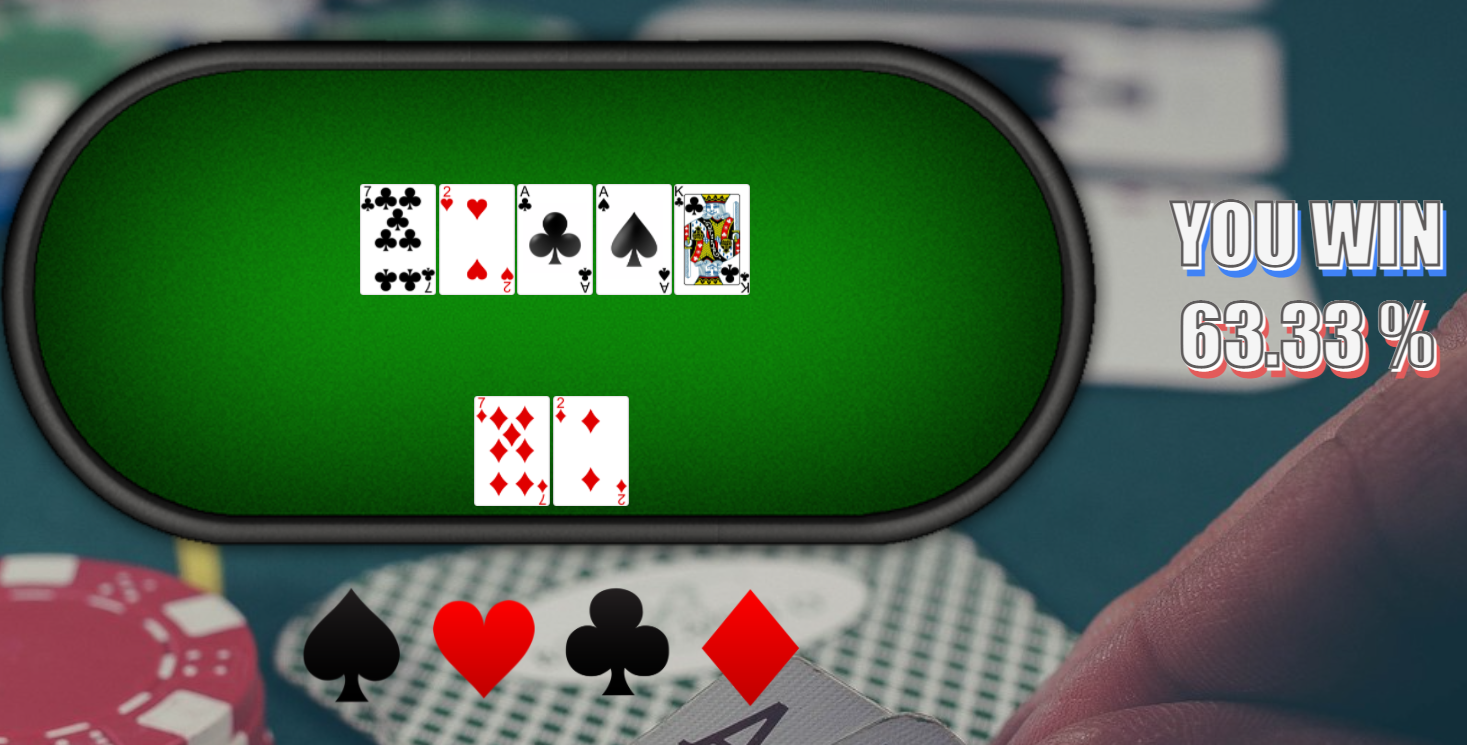
\includegraphics[scale=0.47]{images/test-my.png}
\caption{Az alkalmazásom számítási eredménye river-nél}
\label{fig:test-my}
\end{figure}

A diagramm helyes működésének a vizsgálata már bonyolultabb folyamat. Ebben az esetben azt a megoldást választottam, hogy egy olyan kártyakombinációt választok, amelynek viszonylag egyedi diagrammja lesz. Például turn-nél négy treff van az asztalon, a felhasználó kezében két káró van és sem párt, sem erősebb kezet nem alkotnak a lapok. Ebben az estben, ha még egy pikk érkezne river-nél, akkor a board-on lévő lapok flush-t alkotnának, amit a program nyereségként ábrázol. Tehát a diagrammon azt kell látnunk, hogy a maradék pikk lapok esetén nagyon magas a nyerési esélye a felhasználónak.

\begin{figure}[ht] 
\centering
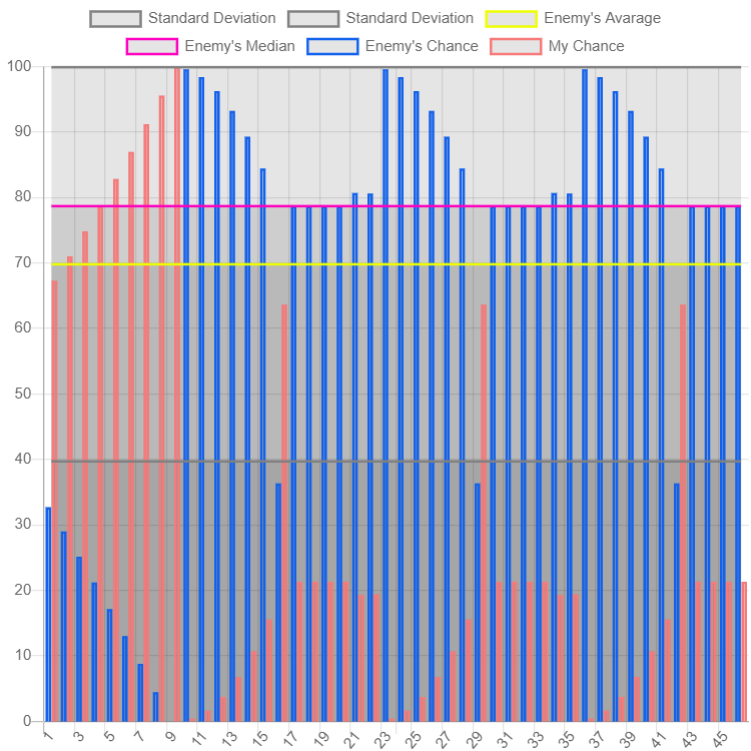
\includegraphics[scale=0.9]{images/chart-test.png}
\caption{A kirajzolt diagramm turn-nél}
\label{fig:chart-test}
\end{figure}

Ennek megfelelően kiválasztottam a felhasználó lapjainak a káró 2-est és 3-mast, az asztalra pedig a treff ászt, királyt, dámát, és bubit. Ezután legeneráltam a diagrammot, ami alább látható. Az everyCards tömbben növekő sorrendben helyezkednek el a lapok, először a treff, majd a káró, kör, végül pedig a pikk. A lapokból az látszik, hogy ha bármelyik treff következik a river-nél, akkor a board-on flush alakulna ki, ha a treff 10-es érkezne, akkor pedig royal flush. Ezen kívül, ha bármilyen 10-es érkezne, akkor sor alakulni ki a boardon, ami szintén a felhasználónak kedvez. A kézben lévő lapok a lehető legalacsonyabbak, illetve nem alakulhat ki belőle flush, sor, de még csak egy drill sem. Ha nem érkezik több treff, akkor a legmagasabb kezünk, ami lehet, az egy hármas pár, viszont ez sem mondható erősnek, mivel az asztalon csupa magas lap van. 

Ezeket a tényeket mutatja be a 4.4-as ábrán kirajzolt diagramm. A piros oszlop a felhasználó nyerési esélyeit mutatják, a kékek pedig az ellenfelét. Jól látszik, hogy az első kilenc kártyánál nagyon magas a nyerési esélye a felhasználónak. Ezek a maradék treff lapok a pakliban, az utolsó pedig a treff 10-es, aminél 100\% az esély a győzelemre. A többi lapra három kivétellel mindegyiknél az ellenfélnek nagyobb az esélye. Ez a három lap a maradék 10-esek a pakliban, amelyekkel sor alakulna ki a boardon. A lila konstans mutatja az ellenfél esélyeinek mediánját, a sárga az átlagát, a szürkék pedig a szórását. Ezek mind segítik a felhasználót a döntéshozásban.